\documentclass[10pt]{article}

%% Packages to use

\usepackage{amsmath,amsfonts,amssymb,tikz}   %% AMS mathematics macros
\usetikzlibrary{shapes.geometric}

\title{CoinJoin Anonymity Analysis}


\begin{document}

\maketitle

\section{Introduction}
CoinJoin is a technique for combining multiple Bitcoin transactions into a single one to make it more difficult for blockchain analyzers to determine which the original transactions are.\\\\ 
In this document we want to keep a record of our attempts to create a general approach for analyzing the pros and cons of the different mixing algorithms.

\section{Mixing}

\label{sec: mixing}
Let's say we have these two transactions:
\label{eqn: mixing}

\begin{center}
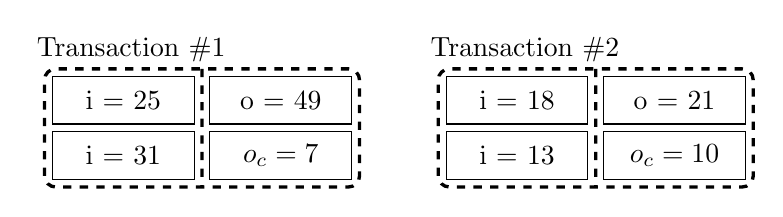
\begin{tikzpicture}[input/.style={rectangle,thin,draw, minimum width=1.8cm, minimum height=0.6cm}]

\draw[dashed, very thick, rounded corners] 
      (0,0) rectangle (4,1.5) (2,1.5) -- (2,0)
      (1.1,1.75) node {Transaction \#1};
\draw (1,1.1) node[input] {i = 25} (3,1.1) node[input] {o = 49}
      (1,0.4) node[input] {i = 31} (3,0.4) node[input] {$o_c = 7$};

\draw[dashed, very thick, rounded corners] 
      (5,0) rectangle (9,1.5) (7,1.5) -- (7,0)
      (6.1,1.75) node {Transaction \#2};
\draw (6,1.1) node[input] {i = 18} (8,1.1) node[input] {o = 21}
      (6,0.4) node[input] {i = 13} (8,0.4) node[input] {$o_c = 10$};
\end{tikzpicture}
\end{center}

They can be combined in one transaction as follow:

\begin{center}
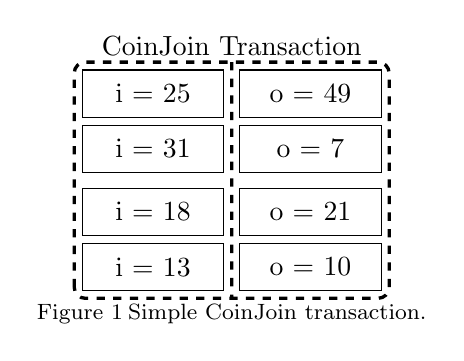
\begin{tikzpicture}[input/.style={rectangle,thin,draw, minimum width=1.8cm, minimum height=0.6cm}]

\draw[dashed, very thick, rounded corners] 
      (0,0) rectangle (4,3) (2,3) -- (2,0)
      (2,3.2) node {CoinJoin Transaction};
      
\draw (1,1.9) node[input] {i = 31} (3,2.6) node[input] {o = 49} 
      (1,2.6) node[input] {i = 25} (3,1.9) node[input] {o = 7}
      (1,1.1) node[input] {i = 18} (3,1.1) node[input] {o = 21} 
      (1,0.4) node[input] {i = 13} (3,0.4) node[input] {o = 10}
      (2, -0.2) node[font=\footnotesize,align=center] {Figure 1\:Simple CoinJoin transaction.};
\end{tikzpicture}
\end{center}

\section{Analysis}

We are going to focus specifically on blockchain analysis where the analysts goal is attach identities to coins (outputs) and tracking them using two well-known heuristics:
 
\begin{itemize}
  \item H1: All inputs to a transaction are owned by the same entity
  \item H2: The  one-time  change  address  is  controlled  by
the same entity as the input addresses
\end{itemize}


These heuristics cannot be applied to CoinJoin transactions but only to single payment transactions instead. For that reason the analysts have to unjoin the coinjoined transactions with the hope of finding the original payment transactions to apply the heuristics individually.\\

Side note: H1 is clearly a more robust assumption than H2.

\subsection{Unjoining coinjoined transactions}
Let's take the coinjoin transaction in figure 1. That transaction can be interpreted in many different ways but, \textit{just for simplicity}, lets assume that we know this is a coinjoin transaction between two (no obvious) participants and that each transaction has no more than two outputs. This is enough for extracting the original transactions by grouping the outputs, the inputs and then match the sum of both sets: \\

Outputs:

\begin{tabular}{| r | c | r | l | r | c | r |}
  \hline			
  \# & OutputSet & Sum(OSet) & & \# & OutputSet & Sum(OSet) \\
  \hline
  0 & \{49\} & 49 & & 5 & \{49, 21\} & 70 \\
  1 & \{7\} & 7 & & 6 & \{49, 10\} & 59 \\
  2 & \{21\} & 21 & & 7 & \{7, 21\} & 28 \\
  3 & \{10\} & 10 & & 8 & \{7, 10\} & 17 \\
  4 & \{49, 7\} & \textbf{56} & & 9 & \{21, 10\} & \textbf{31} \\
  \hline  
\end{tabular}\\\\

Inputs:

\begin{tabular}{| r | c | r | l | r | c | r |}
  \hline			
  \# & InputSet & Sum(ISet) & & \# & InputSet & Sum(ISet) \\
  \hline
  0 & \{25\} & 25 & & 7 & \{31, 18\} & 49 \\
  1 & \{31\} & \textbf{31} & & 8 & \{31, 13\} & 44 \\
  2 & \{18\} & 18 & & 9 & \{18, 13\} & \textbf{31} \\
  3 & \{13\} & 13 & & 10 & \{25, 31, 18\} & 74 \\
  4 & \{25, 31\} & \textbf{56} & & 11 & \{25, 31, 13\} & 69 \\
  5 & \{25, 18\} & 43 & & 12 & \{25, 18, 13\} & \textbf{56} \\
  6 & \{25, 13\} & 38 & & 13 & \{31, 18, 13\} & 62 \\
  \hline  
\end{tabular}\\\\


Before continuing with the example, it worth to note that given the coinjoin transaction has 4 inputs and that we know there are two sub-transaction then, the maximum number of inputs a sub-transaction can have is 3. These 3 inputs can be combined in 14 different ways.
The number of ways a set with of $n$ elements can be partitioned into disjoint subsets is called `Bell number` and it grows rapidly as the value of $n$ increases. \\

Having built this table it is possible now to extract all the possible transactions. In this case we have 4 sub-transactions (\#1, \#2, \#3 and \#4)


\begin{center}
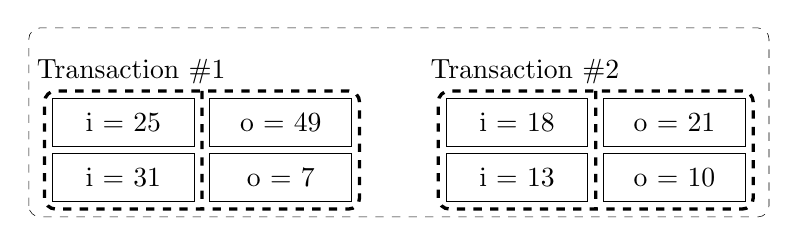
\begin{tikzpicture}[input/.style={rectangle,thin,draw, minimum width=1.8cm, minimum height=0.6cm}]
\draw[dashed, very thin, rounded corners]
      (-0.2,-0.1) rectangle (9.2,2.3);

\draw[dashed, very thick, rounded corners] 
      (0,0) rectangle (4,1.5) (2,1.5) -- (2,0)
      (1.1,1.75) node {Transaction \#1};
\draw (1,1.1) node[input] {i = 25} (3,1.1) node[input] {o = 49}
      (1,0.4) node[input] {i = 31} (3,0.4) node[input] {o = 7};

\draw[dashed, very thick, rounded corners] 
      (5,0) rectangle (9,1.5) (7,1.5) -- (7,0)
      (6.1,1.75) node {Transaction \#2};
\draw (6,1.1) node[input] {i = 18} (8,1.1) node[input] {o = 21}
      (6,0.4) node[input] {i = 13} (8,0.4) node[input] {o = 10};

\end{tikzpicture}
\end{center}

\begin{center}
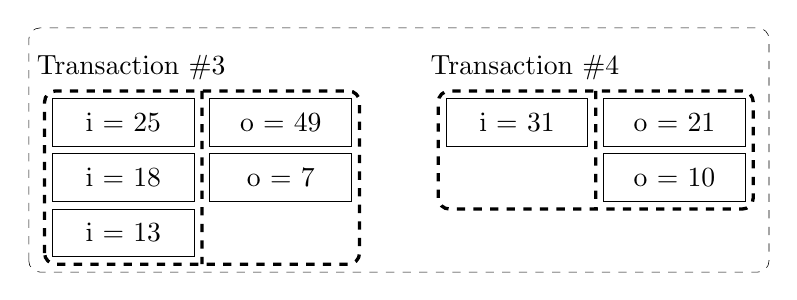
\begin{tikzpicture}[input/.style={rectangle,thin,draw, minimum width=1.8cm, minimum height=0.6cm}]

\draw[dashed, very thin, rounded corners]
      (-0.2,-0.1) rectangle (9.2,3.0);
        
\draw[dashed, very thick, rounded corners] 
      (0,0) rectangle (4,2.2) (2,2.2) -- (2,0)
      (1.1,2.5) node {Transaction \#3};
\draw (1,1.8) node[input] {i = 25} (3,1.8) node[input] {o = 49}
      (1,1.1) node[input] {i = 18} (3,1.1) node[input] {o = 7}
      (1,0.4) node[input] {i = 13};

\draw[dashed, very thick, rounded corners] 
      (5,0.7) rectangle (9,2.2) (7,2.2) -- (7,0.7)
      (6.1,2.5) node {Transaction \#4};
\draw (6,1.8) node[input] {i = 31} (8,1.8) node[input] {o = 21}
                                   (8,1.1) node[input] {o = 10};

\end{tikzpicture}
\end{center}

Also, we can see that if well all of these look perfectly valid, there are only two valid sets of transactions that could result in the original coinjoined transaction and in the image above we had wrapped them together in the dashed boxes. They are

\begin{itemize}
  \item Transaction \#1 and Transaction \#2
  \item Transaction \#3 and Transaction \#4
\end{itemize}


Clearly, other combinations are invalid because same inputs appears in more than one sub-transaction.\\

It is important to note that in this really simple example an analyzer has only 0.5 probability of choosing the right original sub-transactions set. In practice this does not use to happen but the good part is that we can make it happen simply by choosing the outputs values (that's what knapsack and traditional coinjoins do).

\subsection{Equal-output coinjoin comparison}

Lets say two people want to coinjoin together to obtain coins of the exact same value (for this example lets say 10). Both provide their transactions:


\begin{center}
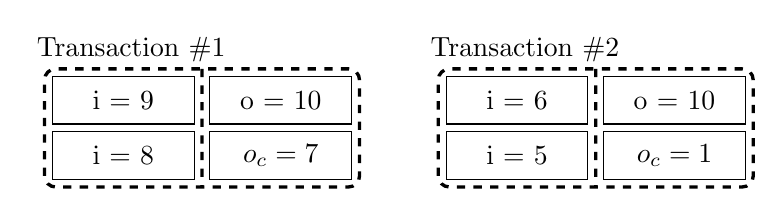
\begin{tikzpicture}[input/.style={rectangle,thin,draw, minimum width=1.8cm, minimum height=0.6cm}]

\draw[dashed, very thick, rounded corners] 
      (0,0) rectangle (4,1.5) (2,1.5) -- (2,0)
      (1.1,1.75) node {Transaction \#1};
\draw (1,1.1) node[input] {i = 9} (3,1.1) node[input] {o = 10}
      (1,0.4) node[input] {i = 8} (3,0.4) node[input] {$o_c = 7$};

\draw[dashed, very thick, rounded corners] 
      (5,0) rectangle (9,1.5) (7,1.5) -- (7,0)
      (6.1,1.75) node {Transaction \#2};
\draw (6,1.1) node[input] {i = 6} (8,1.1) node[input] {o = 10}
      (6,0.4) node[input] {i = 5} (8,0.4) node[input] {$o_c = 1$};
\end{tikzpicture}
\end{center}

After join them, they get the following transaction:

\begin{center}
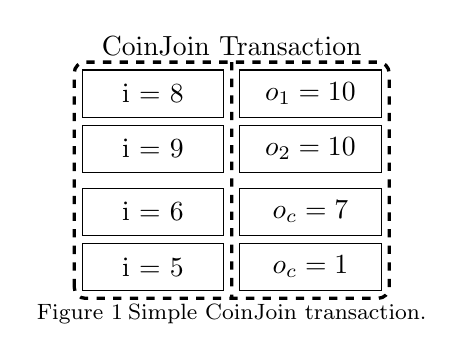
\begin{tikzpicture}[input/.style={rectangle,thin,draw, minimum width=1.8cm, minimum height=0.6cm}]

\draw[dashed, very thick, rounded corners] 
      (0,0) rectangle (4,3) (2,3) -- (2,0)
      (2,3.2) node {CoinJoin Transaction};
      
\draw (1,1.9) node[input] {i = 9} (3,2.6) node[input] {$o_1 = 10$} 
      (1,2.6) node[input] {i = 8} (3,1.9) node[input] {$o_2 = 10$}
      (1,1.1) node[input] {i = 6} (3,1.1) node[input] {$o_c = 7$} 
      (1,0.4) node[input] {i = 5} (3,0.4) node[input] {$o_c = 1$}
      (2, -0.2) node[font=\footnotesize,align=center] {Figure 1\:Simple CoinJoin transaction.};
\end{tikzpicture}
\end{center}

This coinjoin transaction can be analyzed in the same way that we did before but in this case we don't need some of the assumptions that we used then because unlike the naïve coinjoin transaction we used initially, this transaction has a clear fingerprint and it is easy to know the number of participants involved simply by counting the number of indistinguishable outputs. Also, the change outputs are clearly identifiable. Finally, extracting the possible sub-transactions is trivial and doesn't require building big tables as before. Just take a change value, add it 10 and look what inputs sum gives us that result.

\begin{center}
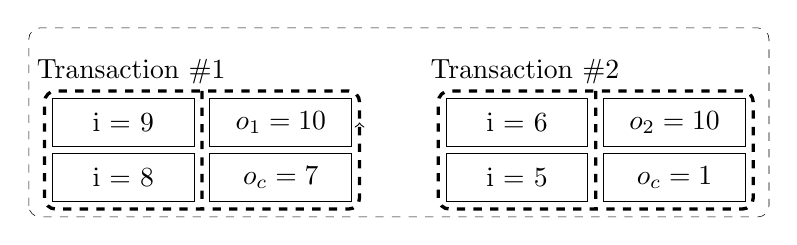
\begin{tikzpicture}[input/.style={rectangle,thin,draw, minimum width=1.8cm, minimum height=0.6cm}]
\draw[dashed, very thin, rounded corners]
      (-0.2,-0.1) rectangle (9.2,2.3);

\draw[dashed, very thick, rounded corners] 
      (0,0) rectangle (4,1.5) (2,1.5) -- (2,0)
      (1.1,1.75) node {Transaction \#1};
\draw (1,1.1) node[input] {i = 9} (3,1.1) node[input] {$o_1 = 10$}
      (1,0.4) node[input] {i = 8} (3,0.4) node[input] {$o_c = 7$}
      (3, 1.1)[->] (4,1.1);

\draw[dashed, very thick, rounded corners] 
      (5,0) rectangle (9,1.5) (7,1.5) -- (7,0)
      (6.1,1.75) node {Transaction \#2};
\draw (6,1.1) node[input] {i = 6} (8,1.1) node[input] {$o_2 = 10$}
      (6,0.4) node[input] {i = 5} (8,0.4) node[input] {$o_c = 1$};

\end{tikzpicture}
\end{center}

\begin{center}
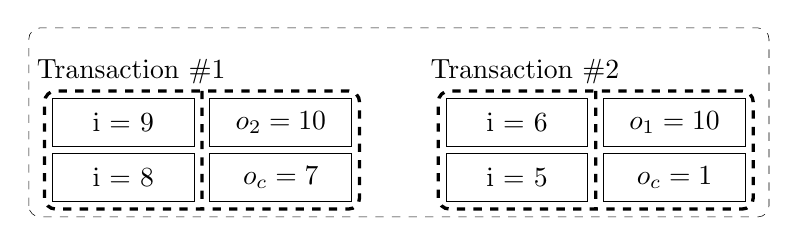
\begin{tikzpicture}[input/.style={rectangle,thin,draw, minimum width=1.8cm, minimum height=0.6cm}]
\draw[dashed, very thin, rounded corners]
      (-0.2,-0.1) rectangle (9.2,2.3);

\draw[dashed, very thick, rounded corners] 
      (0,0) rectangle (4,1.5) (2,1.5) -- (2,0)
      (1.1,1.75) node {Transaction \#1};
\draw (1,1.1) node[input] {i = 9} (3,1.1) node[input] {$o_2 = 10$}
      (1,0.4) node[input] {i = 8} (3,0.4) node[input] {$o_c = 7$};

\draw[dashed, very thick, rounded corners] 
      (5,0) rectangle (9,1.5) (7,1.5) -- (7,0)
      (6.1,1.75) node {Transaction \#2};
\draw (6,1.1) node[input] {i = 6} (8,1.1) node[input] {$o_1 = 10$}
      (6,0.4) node[input] {i = 5} (8,0.4) node[input] {$o_c = 1$};

\end{tikzpicture}
\end{center}

We can see in this example that the equal-outputs coinjoin transaction provides 0.5 probability to track the "anonymized" coin. 



\end{document}

